Minwise-Hashing or MinHash LSH is one of the methods of LSH, it was proposed to
estimate the Jaccard similarity metric  between data points of any sizes. It
relies on the fact that applying a random permutation to the set of data points,
the chance that the smallest item under this permutation in sets $A$ and $B$ are
precisely the same as their similarity of Jaccard. \citep{yu_yun_2022}

\subsubsection{Formulation}
The classic formulation of MinHash was to use a set of permutations over the
data points, and take the argument corresponding to the minimum value of each
permuted column (or corresponding to the first occurrence of 1 in case of binary
data).

Knowing that the permutations consume lot of memory when the number of data
points get bigger, it becomes more complicated to use them. A new formulation
has occurred, where each set is converted to a MinHash signature using a set of
$m$ minwise-hashing functions $(h_{min_1}, h_{min_2}, \cdot, h_{min_m})$. A
minwise-hashing function's value $h_{min}(X)$ of a set $X$ is obtained by taking
the minimum from the result of applying a set of independently generated hashing
functions $(h_1,h_2, .., h_l)$ on a column: $h_{min}(X) = min(h_1(X), h_2(X),
    \cdot, h_l(X))$ \citep{zhu_lshensemble_2016}. Each function $h_i$ will then
return an integer value. Each column will have a value for each of the $m$
minwise-hashing functions which is its hash value, and the column can be
represented by the concatenation of its hash values, the concatenation that is
also called the column signature. The signature matrix is the concatenation of
the columns signatures, and it will be on size $(m,d)$.

\begin{figure}[h]
    \centering
    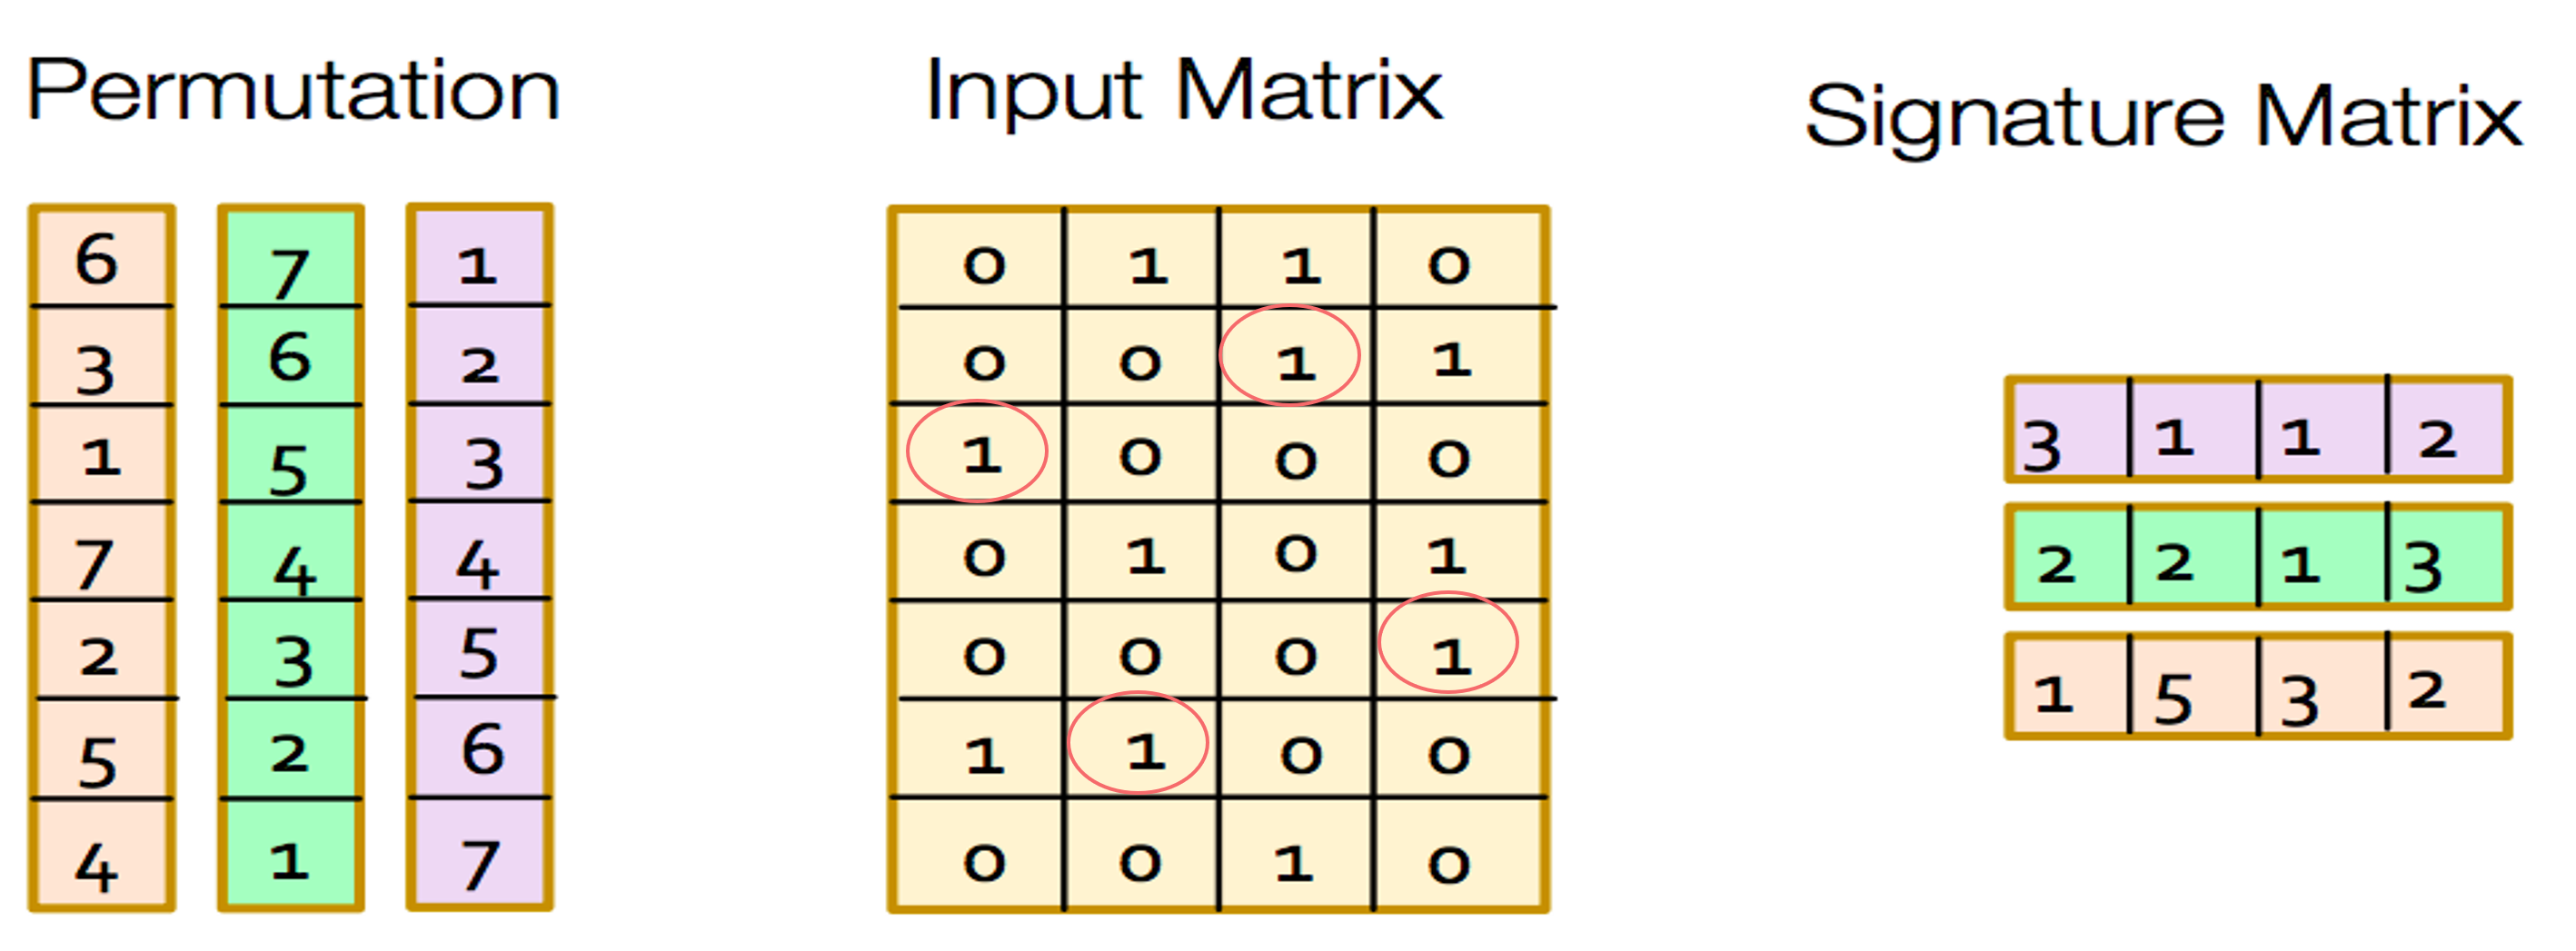
\includegraphics[width=\textwidth]{state_of_the_art/methods/minhash_example.png}
    \caption{Minwise-Hashing LSH example}
    \label{fig:minhashing_example}
\end{figure}

The figure \ref{fig:minhashing_example} shows an example on hashing with MinHash LSH.

When applied on a data matrix of size ($n, d$), MinHash LSH has a time
complexity of $O(m \; log\;m + n)$; where $m$ is the number of hash functions.
\citep{ertl_2020}

The main advantage of MinHash LSH is its suitability for discrete sets of data
as it relies on the Jaccard similarity which is an accurate measurement for this
type of data. On the other hand, MinHash LSH is less suitable when it comes to
treating and detecting similarities between continuous datasets (data with real
numbers for example), and this is again related to the measure that it tries to
estimate (Jaccard similarity), which is not accurate in this case.
